% Russian counterpart of the journal-neutral manuscript. Edit directly.
\documentclass[11pt,a4paper]{article}
\usepackage[T2A]{fontenc}
\usepackage[utf8]{inputenc}
\usepackage[english,russian]{babel}
\usepackage[margin=25mm]{geometry}
\usepackage{amsmath,amssymb,graphicx}
\usepackage[numbers,sort&compress]{natbib}
\usepackage[hyphens]{url}
\usepackage[hidelinks]{hyperref}
\ifx\pdfmapfile\undefined\else
\pdfmapfile{+cm-super-t1.map}\pdfmapfile{+cm-super-t2a.map}
\pdfmapfile{+cm-super-ts1.map}\fi
\setlength{\emergencystretch}{2em}
\renewcommand{\topfraction}{0.85}
\renewcommand{\textfraction}{0.10}
\renewcommand{\floatpagefraction}{0.75}

\title{Передача напряжений и движение дислокаций в алюминии
вблизи включения Al$_{13}$Fe$_4$ с удерживаемой деформацией}
\author{И.\,Е.~Михайловский\thanks{Автор для переписки.
\texttt{ilyamihailovsy@gmail.com}} \and Д.\,Е.~Пшонкин}
\date{Московский политехнический университет, Москва, Россия}

\begin{document}
\maketitle

\begin{abstract}
Атомистическим методом исследован механический отклик алюминия на заданную
деформацию включения Al$_{13}$Fe$_4$. В ячейке границы из 91\,428 атомов
выступ включения удлинён на 0{,}194\% и удерживается при релаксации матрицы.
Модуль дополнительного касательного напряжения над осью выступа достигает
15{,}45~МПа; усреднение по ширине ячейки приводит к существенной
компенсации напряжений. В парных расчётах под нагрузкой уход существующей
верхней дислокации зарегистрирован при 113{,}6~МПа в контроле и
122{,}7~МПа при деформированном выступе. Начальное движение и остаточные
сегменты на периодическом шве ограничивают интерпретацию этой разницы.
Отдельная модель термически активированного скольжения показывает
чувствительность ползучести к принятой амплитуде напряжений и активационному
объёму. Установленный механический отклик относится к заданному условию
удержания. Магнитная деформация включений и сохранение эффекта после
снятия поля в этих расчётах не проверены.
\end{abstract}

\noindent\textbf{Ключевые слова}\quad молекулярная динамика; межфазные
напряжения; дислокации; алюминиевые сплавы; удерживаемая деформация

\section{Введение}

Изменение пластических свойств алюминиевых сплавов после магнитной
обработки ставит вопрос о механическом взаимодействии включений с
дислокациями. В экспериментах с неоднородными сплавами Al--Mg--Si,
содержащими железосодержащие включения, обнаружены изменения ползучести
после выдержки в постоянном поле
\cite{Skvortsov2019JAP,Skvortsov2019PSS,Friha2024JMMM}.
Магнитная обработка и механическое нагружение в этих опытах были
разделены во времени. В последующей работе также отмечены изменения
переходных стадий ползучести и релаксации напряжений
\cite{Nikolaev2025SciRep}. Объяснение сохраняющегося отклика поэтому
требует установить, какое состояние материала остаётся после
завершения обработки.

Возможный вклад связан с напряжениями, возникающими при изменении формы
включения внутри матрицы. Источником деформации может быть
магнитострикция, если включение содержит соответствующую магнитную фазу.
Механический отклик зависит от формы частицы, упругой податливости
окружения и кристаллографической ориентации. Скалярная оценка напряжения
на границе сама по себе не определяет сдвиг, действующий на конкретную
дислокацию. На движение линии вблизи включения также влияют исходное
поле границы и распределение препятствий.

В настоящей работе исследуется механическая часть этой задачи для
алюминиевой матрицы с включением Al$_{13}$Fe$_4$. Заданное удлинение
0{,}194\% определяет амплитуду контролируемого возмущения. Оно следует
из модельной оценки, связанной с принятой ранее шкалой напряжений
147~МПа \cite{Friha2024JMMM}; деформация включений такой величины
в магнитном поле непосредственно не измерена. Наложенные ограничения
удерживают опорные координаты атомов включения. Полученное поле
соответствует определённому механическому граничному условию.
Для отождествления этого условия с магнитным превращением нужны
дополнительные основания.

Парный статический расчёт напряжений сопоставляется с траекториями
существующих дислокаций в той же геометрии границы. Отдельно
рассматриваются касательное напряжение со знаком вблизи оси включения
и средние значения по ширине ячейки. При анализе траекторий учитываются
начальная релаксация, последующее движение и взаимодействие линий
с периодическим швом. Затем отдельная модель термически активированного
скольжения связывает принятые амплитуды напряжений с условным
изменением скорости ползучести. Такая постановка позволяет определить
рассчитанный отклик и пределы его интерпретации, не приписывая
экспериментальному эффекту памяти установленный микроскопический механизм.

\section{Методика}

\subsection{Геометрия и заданная деформация}

Расчёты выполнены в LAMMPS версии от 22 июля 2025 г. с ускорением
KOKKOS/CUDA \cite{Thompson2022LAMMPS}. Межатомное взаимодействие задано
потенциалом модифицированного метода погружённого атома с учётом
вторых соседей для Al--Si--Mg--Cu--Fe \cite{Jelinek2012}.
Гранецентрированная кубическая решётка алюминия имеет параметр
$a_0=4{,}05$~\AA{} и ориентацию
$x\parallel[1\bar{1}0]$, $y\parallel[11\bar{2}]$,
$z\parallel[111]$. При таком выборе плоскость скольжения (111)
параллельна номинальной границе, а направление скольжения
$[1\bar{1}0]$ совпадает с $x$. Краевая дислокация с линией вдоль $y$
имеет вектор Бюргерса $\mathbf b=(a_0/2)[1\bar{1}0]$,
$b=2{,}864$~\AA{}.

Моноклинный Al$_{13}$Fe$_4$ \cite{Liu2024CIF} образует опорный слой
толщиной 20~\AA{} с полуэллиптическим выступом. Полуоси сечения
выступа равны 35~\AA{} вдоль $x$ и 20~\AA{} вдоль $z$; он проходит
через ячейку в периодическом направлении $y$. Каждая ячейка границы
содержит 91\,428 атомов, из которых 72\,532 относятся к матрице и
18\,896 к включению. Размеры в плоскости составляют
$154{,}64\times64{,}48$~\AA$^2$. Вдоль $x$ и $y$ действуют
периодические условия, верхняя поверхность алюминия обращена в вакуум,
нижние 6~\AA{} закреплены. Геометрия представлена на
рис.~\ref{fig:model}. Связь фаз и возможная атомная перестройка
границы определяются межатомным потенциалом.

\begin{figure}[!htbp]
\centering
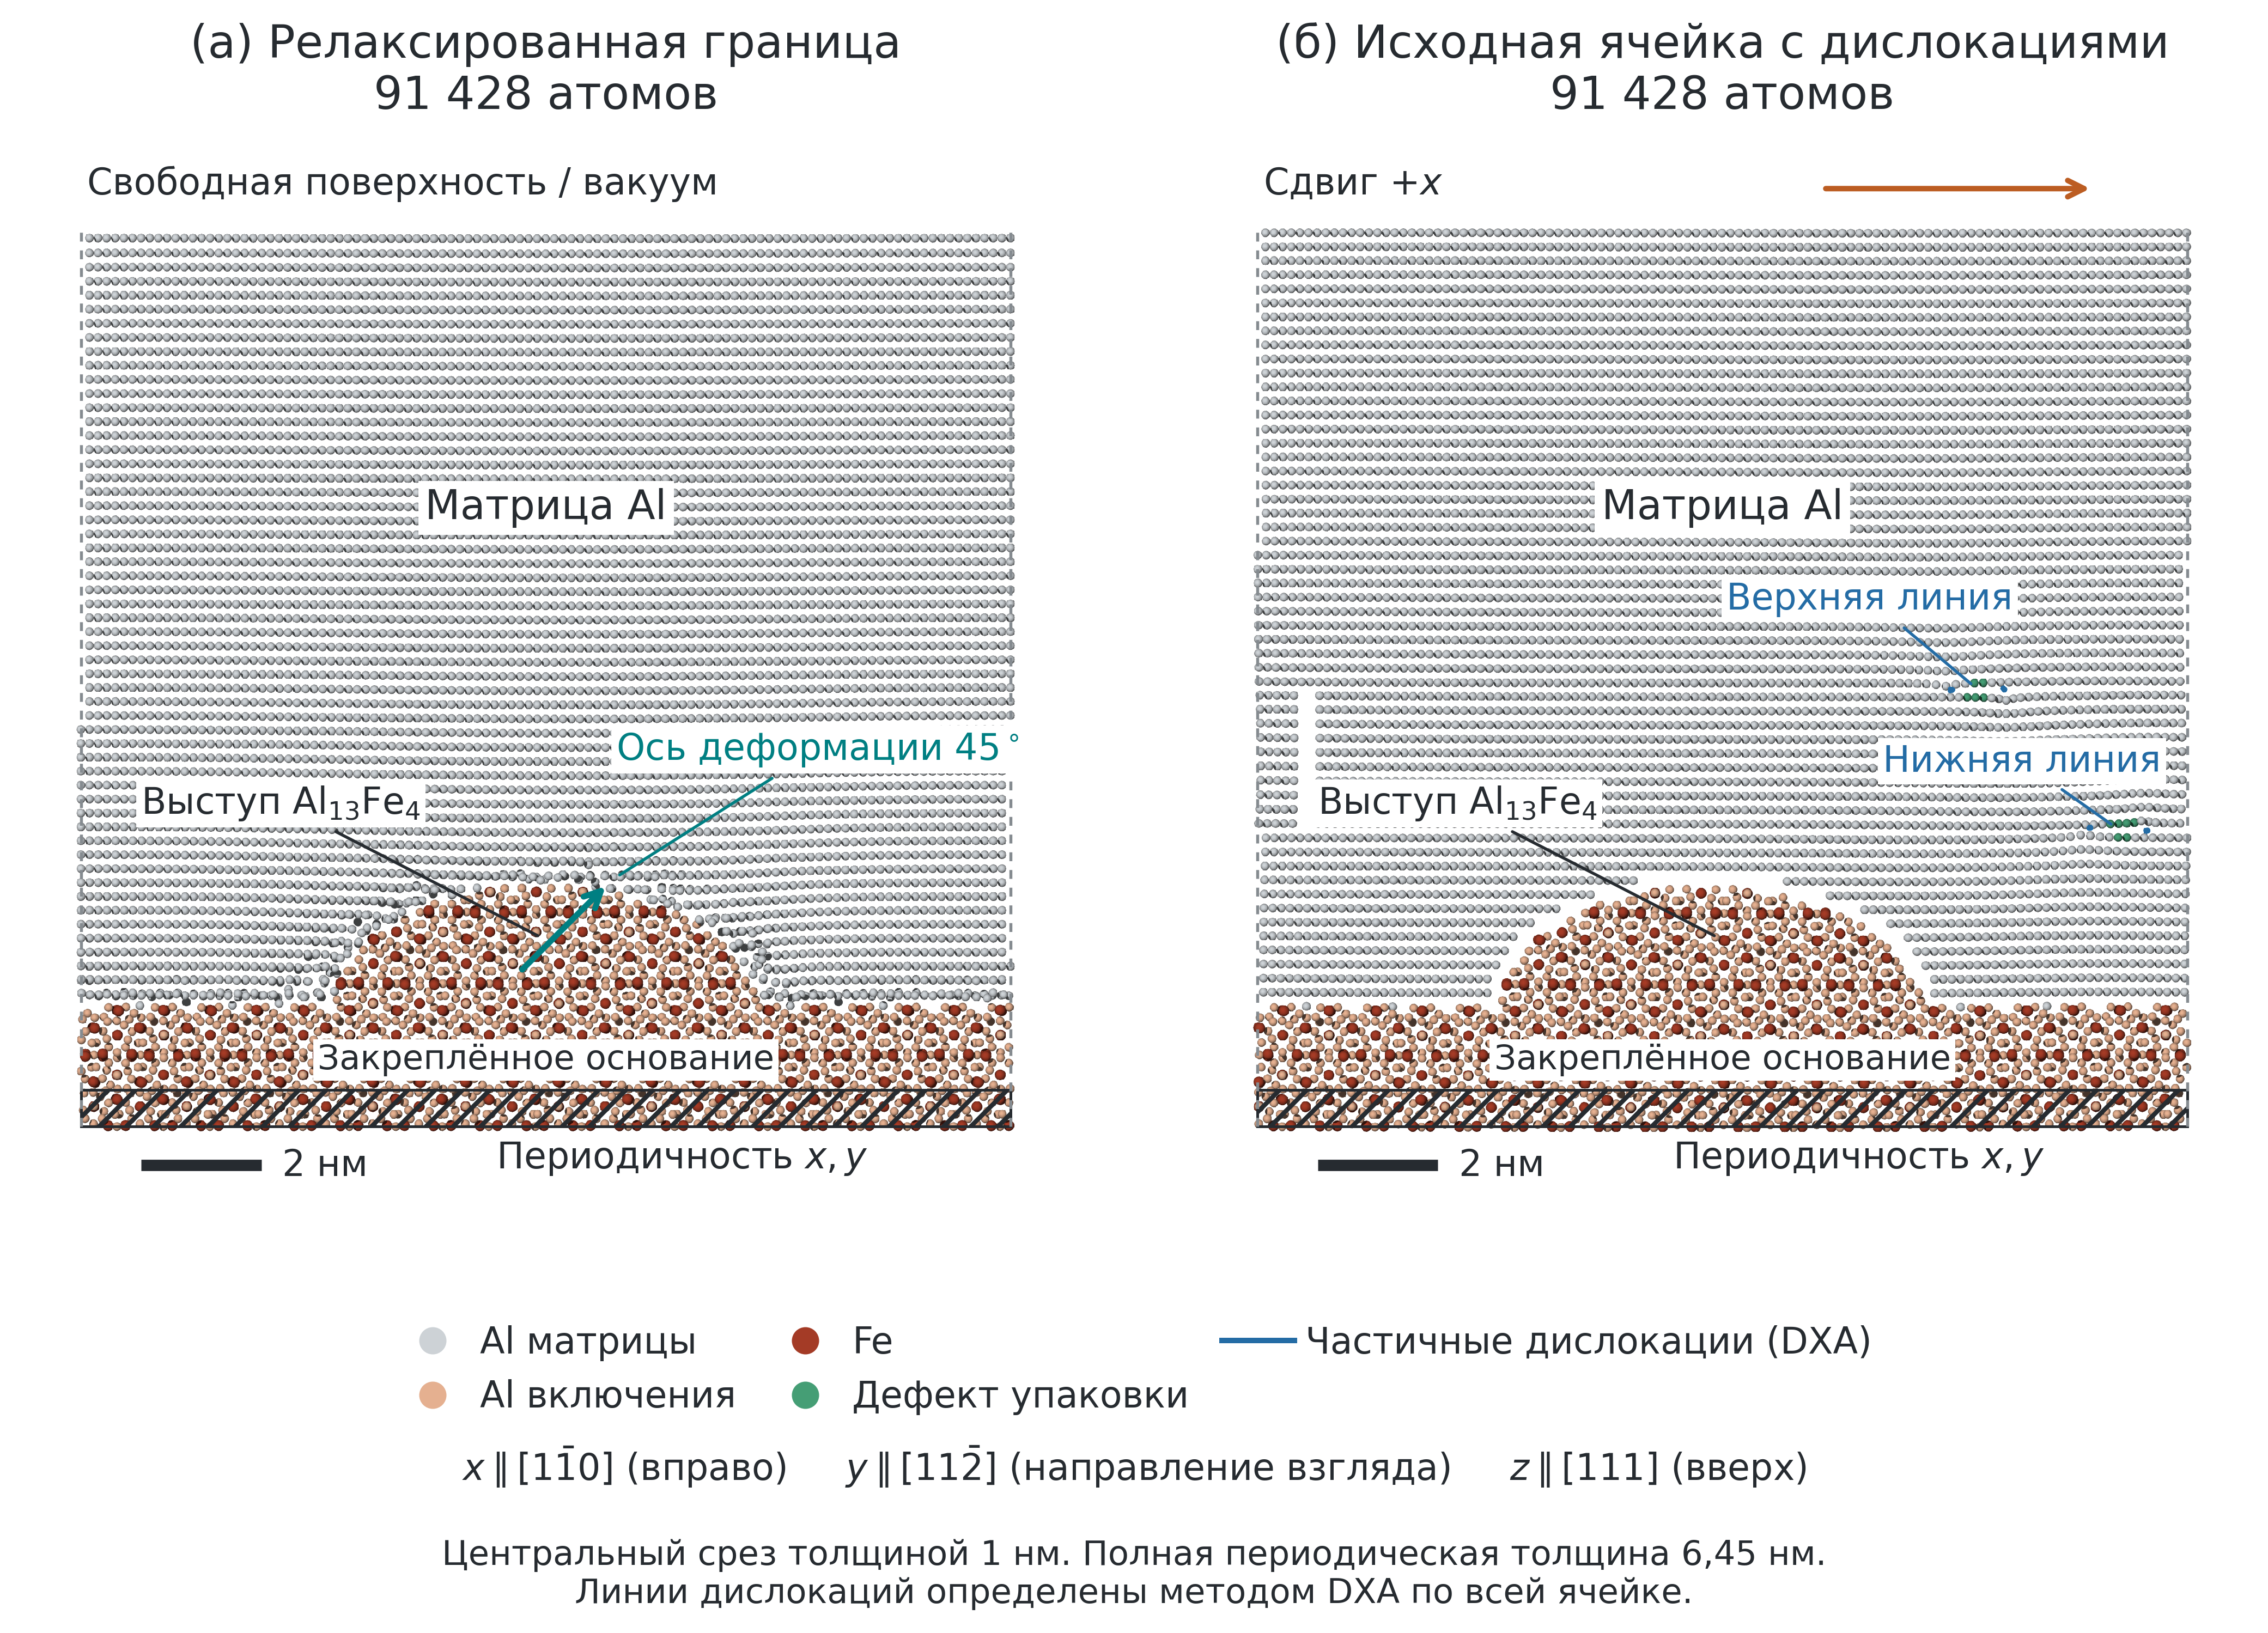
\includegraphics[width=0.92\linewidth]{fig_model_ru.png}
\caption{Атомистическая геометрия границы, визуализированная в OVITO
по конфигурациям LAMMPS. Выступ Al$_{13}$Fe$_4$ протянут вдоль $y$
над плоским опорным слоем. Оси соответствуют направлению скольжения,
направлению линии и нормали к границе. Нагружаемая конфигурация
содержит пару краевых дислокаций противоположного знака. Верхние слои
передают сдвиговую нагрузку, нижний слой закреплён.}
\label{fig:model}
\end{figure}

Атомы выступа смещаются относительно его центра с использованием
тензора малой деформации
\begin{equation}
\mathbf E_0=\frac{3\varepsilon_0}{2}
 \left(\mathbf u\otimes\mathbf u-\frac{\mathbf I}{3}\right),
\qquad
\varepsilon_0=0{,}00194,\qquad
\mathbf u=\frac{(1,0,1)}{\sqrt{2}} .
\label{eq:strain}
\end{equation}
Нулевой след обеспечивает сохранение объёма в первом порядке.
Выбранное направление максимизирует компоненту $xz$ в этом семействе
деформаций, $E_{0,xz}=0{,}001455$, и представляет одну благоприятную
ориентацию. Опорному слою начальное смещение не задаётся.

Из предварительно релаксированной структуры готовятся контрольная
и возмущённая копии, которые минимизируются при одинаковых настройках.
Атомы включения связаны с соответствующими опорными координатами
гармоническими пружинами жёсткостью 20~эВ/\AA$^2$.
Матрица свободно релаксирует. Межатомный потенциал остаётся прежним,
поэтому необходимые для удержания деформации силы создаются
ограничениями. Собственная деформация материала означала бы изменение
его ненапряжённого состояния. Реакции пружин входят в парный отклик
при одинаковой жёсткости в обоих расчётах. Подготовка конфигураций
и сведения о сходимости приведены в дополнительных материалах.

Подготовка включает минимизацию методом сопряжённых градиентов,
6~пс при 300~К, охлаждение до 0{,}5~К за 12~пс и заключительную
минимизацию. Статическая пара затем строится из одного подготовленного
контроля с сохранением соответствия атомных идентификаторов.
В обеих копиях отдельная минимизация достигает заданной
евклидовой нормы сил 0{,}02~эВ/\AA{}. Парная подготовка уменьшает
различия, связанные с независимой релаксацией границ. Устойчивость
к выбору начальной структуры и допуска минимизации этим не
устанавливается; сравнение относится к одному подготовленному состоянию.

\subsection{Определение напряжений и движения дислокаций}

Шесть компонент конфигурационного атомного вириала усредняются
до вычисления инвариантов напряжений. При пересчёте используется
атомный объём алюминия 16{,}61~\AA$^3$. Профиль представляет разность
тензоров возмущённой и контрольной ячеек,
$\Delta\boldsymbol\sigma=\boldsymbol\sigma_\varepsilon-
\boldsymbol\sigma_0$, в слоях толщиной 4~\AA{}. Нормальные напряжения
считаются положительными при сжатии. Знак тензора противоположен
соглашению Коши с положительным растяжением; модули проекций сдвига
и инварианты от этого не меняются.
Координата $r=z-20$~\AA{} отсчитывается от номинальной плоской
границы; $d=r-20$~\AA{} обозначает высоту над номинальной вершиной
выступа. Для слоя, проходящего через всю ячейку, $d$ не является
кратчайшим расстоянием до поверхности включения.

Сохраняются два пространственных средних, по полной ширине ячейки
и по окну $|x-x_c|<10$~\AA{} вблизи оси выступа.
Слои, пересекающие включение, исключены из профиля матрицы.
Касательное напряжение со знаком на системе $(111)[1\bar{1}0]$
равно $\Delta\sigma_{xz}$. Дополнительная скалярная величина
$\mathrm{RSS}_{\max}$ определяется как максимум
$|\mathbf s\cdot\Delta\boldsymbol\sigma\mathbf n|$
по двенадцати системам скольжения ГЦК-решётки. Здесь $\mathbf s$
и $\mathbf n$ являются единичными векторами направления скольжения
и нормали к его плоскости.

Принадлежность слою и осевому окну определяется по координатам
контроля и применяется к тем же атомным идентификаторам в обеих
конфигурациях. Это сохраняет состав выборки при смещении атомов
через границы слоёв. Учитываемые слои целиком находятся выше
всех атомов включения в обоих снимках и содержат только алюминий
матрицы, определяемый по идентификаторам атомов.
Тепловой кинетический вклад в минимизированные профили не входит.
Напряжение фон Мизеса разностного тензора и разность двух
напряжений фон Мизеса являются разными величинами;
сдвиговой инвариант возмущения описывает первая из них.

Нагружаемые ячейки границы также содержат 91\,428 атомов.
Две краевые линии противоположного знака вводятся на параллельных
плоскостях скольжения, разделённых расстоянием 23{,}4~\AA{},
с таким же начальным смещением по горизонтали. Их положение
определяется алгоритмом выделения дислокаций DXA
\cite{Stukowski2012DXA} в OVITO \cite{Stukowski2010OVITO}.
Динамика рассчитывается с шагом 1~фс и термостатом Нозе--Гувера
при 300~К. После 5~пс без приложенного сдвига силы на верхних
атомных слоях возрастают по программе с плавным выходом на постоянную
скорость нагружения в течение 16~пс. Парные расчёты с удерживаемым
включением заканчиваются при номинальном напряжении 145{,}45~МПа.
Дополнительный контрольный расчёт с недеформированным свободным
включением продолжается до 400~МПа. Анализируемые кадры сохранены
через 2~пс, что соответствует примерно 9{,}09~МПа на линейном
участке программы.

Для положений линий снимается периодическая неоднозначность вдоль
$x$, а сегменты объединяются по семейству вектора Бюргерса.
Для отдельной линии линейный базовый тренд подбирается по доступным
положениям начиная с 4~пс при номинальном напряжении ниже 40~МПа.
Уход требует отклонения более шести стандартных отклонений
остатков базового тренда, но не менее 8~\AA{}, с сохранением
отклонения в двух следующих позициях наблюдения. Сохранённый
детектор также допускает отсутствие линии в следующем кадре.
Поэтому численный критерий рассматривается вместе с непрерывностью
линии, особенно при достижении периодического шва.
Приводимые интервалы задаются частотой записи и не являются
доверительными интервалами.

Для сопоставления подвижности используется отдельная ячейка сплава
из 92\,800 атомов. Она содержит 1{,}0~ат.\% Mg и 0{,}6~ат.\% Si
и не содержит включения. Её отличающаяся геометрия и ступенчатое
нагружение описаны в дополнительных материалах. Этот расчёт
не входит в парное сравнение ячеек границы.

\section{Результаты}

\subsection{Напряжения в матрице}

Исходная граница несёт значительные остаточные напряжения.
В ближайшем учитываемом слое при $d=2$~\AA{} напряжение фон Мизеса
в контроле составляет примерно 850~МПа. В следующих трёх слоях
оно равно 106, 185 и 157~МПа. Такие пространственные средние атомистических
напряжений характеризуют построенную границу и её релаксированную
структуру. Их величину нельзя непосредственно приравнять
к макроскопическому пределу текучести при одноосном нагружении.
Немонотонность профиля вблизи границы также затрудняет выделение
единственной длины затухания по абсолютному напряжению.

Заданное возмущение создаёт меньшую добавку к этому фону
(рис.~\ref{fig:field}).
Касательное напряжение в осевом окне отрицательно по всему
учитываемому профилю и достигает $-15{,}451$~МПа при $d=22$~\AA{}.
Его модуль составляет около 11--15~МПа в исследованном интервале
$d=2$--30~\AA{}, затем снижается до 10{,}258~МПа при 46~\AA{},
5{,}139~МПа при 66~\AA{} и 1{,}905~МПа при 86~\AA{}.
Эти значения описывают пространственное ослабление напряжения
в минимизированной конфигурации. Время релаксации по ним не определяется.

При усреднении по полной ширине сдвиг преимущественно положителен
и достигает 5{,}042~МПа при $r=50$~\AA{}. Отличие знака и величины
показывает зависимость измеряемой механической характеристики
от области усреднения. При $r=46$~\AA{} средняя компонента $xz$
почти компенсируется, а $\mathrm{RSS}_{\max}=0{,}558$~МПа
соответствует системе $(111)[01\bar{1}]$. В ближайшем слое
при $r=22$~\AA{} выбирается система $(1\bar{1}\bar{1})[101]$,
для которой $\mathrm{RSS}_{\max}=5{,}651$~МПа является наибольшим
значением по ширине ячейки. В остальных слоях максимум относится
к $(111)[1\bar{1}0]$.
Локальный минимум поэтому отчасти связан с проекцией тензора
и пространственным усреднением.

\begin{figure}[!htbp]
\centering
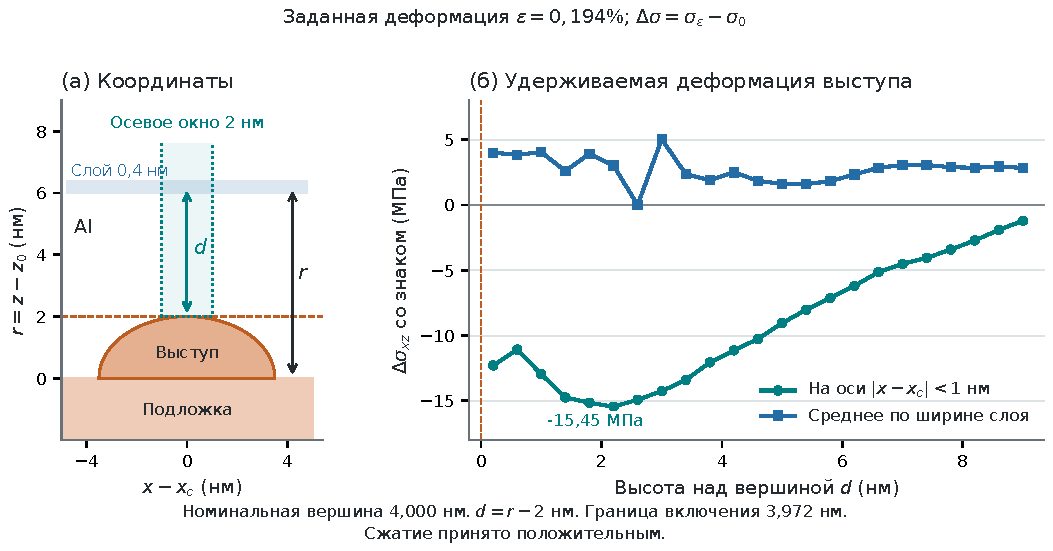
\includegraphics[width=0.96\linewidth]{fig_field_ru.pdf}
\caption{Отсчёт расстояния и касательное напряжение со знаком
в парных минимизированных конфигурациях. На координатной схеме
$r$ отсчитывается от плоской границы, $d$ от номинальной вершины
выступа при $z=40$~\AA{}. Профили сопоставляют
$\Delta\sigma_{xz}$ в осевом окне шириной 20~\AA{}
и среднее по полной ширине ячейки. Учитываются только слои,
нижняя граница которых выше всех атомов включения в обоих снимках
($z_{\max}=39{,}719$~\AA{}). Используется соглашение с положительным
сжатием. Противоположные знаки показывают
зависимость определяемого напряжения от области усреднения.}
\label{fig:field}
\end{figure}

В тринадцати слоях при $r>60$~\AA{} среднее значение
$\mathrm{RSS}_{\max}$ по ширине равно 2{,}477~МПа,
стандартное отклонение составляет 0{,}543~МПа.
Это пространственная статистика одной конфигурации, которая
не даёт независимой оценки численного шума или предела обнаружения.
Небольшой подъём среднего по ширине на большем расстоянии
сопровождается дальнейшим уменьшением модуля сдвига на оси.
На профиль могут влиять конечная толщина слоя и свободная
поверхность; имеющийся расчёт не разделяет их вклады.
Расстояние полного исчезновения поля не определяется.

Линейное преобразование, подобранное по железной подрешётке
выше опорного слоя, даёт проекцию 0{,}9728 на заданную деформацию
выступа с формальной стандартной ошибкой 0{,}0038.
Таким образом, при релаксации матрицы пружины удерживают
большую часть выбранной деформации. Ошибка подгонки характеризует
остатки внутри одной конфигурации и не описывает разброс
между независимыми расчётами. Для континуального сопоставления
использована сферическая частица с тем же номинальным тензором
и одинаковыми изотропными упругими постоянными внутри и снаружи.
Максимальное разрешённое касательное напряжение внутри неё
равно 41{,}45~МПа \cite{Eshelby1957}. Эта отдельная краевая задача
задаёт характерный масштаб напряжений. Верхней оценки для
атомистического выступа она не даёт, поскольку опорный слой,
свободная поверхность и реакции пружин в сферической модели отсутствуют.

\subsection{Существующие дислокации под нагрузкой}

Положение введённых линий меняется в начале всех трёх программ
нагружения. На рис.~\ref{fig:dynamics} показаны парные истории
верхней линии при удерживаемом включении. В контрольной ячейке
со свободным включением верхняя линия за первые 6~пс смещается
примерно на 38~\AA{} к оси выступа. При удерживаемом включении
соответствующие смещения в контрольной и возмущённой ячейках
составляют 31{,}0 и 33{,}2~\AA{}. Верхняя линия оказывается
на расстоянии около 7--10~\AA{} от оси. Нагрузка включается
на 5-й пс, поэтому это начальное движение приходится
преимущественно на предварительную выдержку и плавное начало
нагружения.

Эти смещения показывают, что введённая пара не находится
в стационарном состоянии в исходном окружении. На неё действуют
остаточные напряжения границы, взаимодействие линий,
периодические образы и граничные силы. В обеих ячейках
с удерживаемым включением начальное движение существенно,
поэтому последующий отклик необходимо оценивать относительно
установившихся положений. Начальный интервал сам по себе
не выделяет движение, вызванное только деформацией выступа.

Для верхней линии отклонение от её тренда при малой нагрузке
зарегистрировано при 113{,}6~МПа в контроле и 122{,}7~МПа
в возмущённой ячейке. Предыдущим кадрам соответствуют
104{,}5 и 113{,}6~МПа. Критерий, следовательно, пересекается
в соседних интервалах наблюдения. Для каждой конфигурации
имеется одна траектория при одной скорости нагружения.
Этого недостаточно для определения величины и воспроизводимости
сдвига порога, связанного с деформацией. Статистическое отсутствие
эффекта или критическое напряжение материала из такого сравнения
не следует.

\begin{figure}[!htbp]
\centering
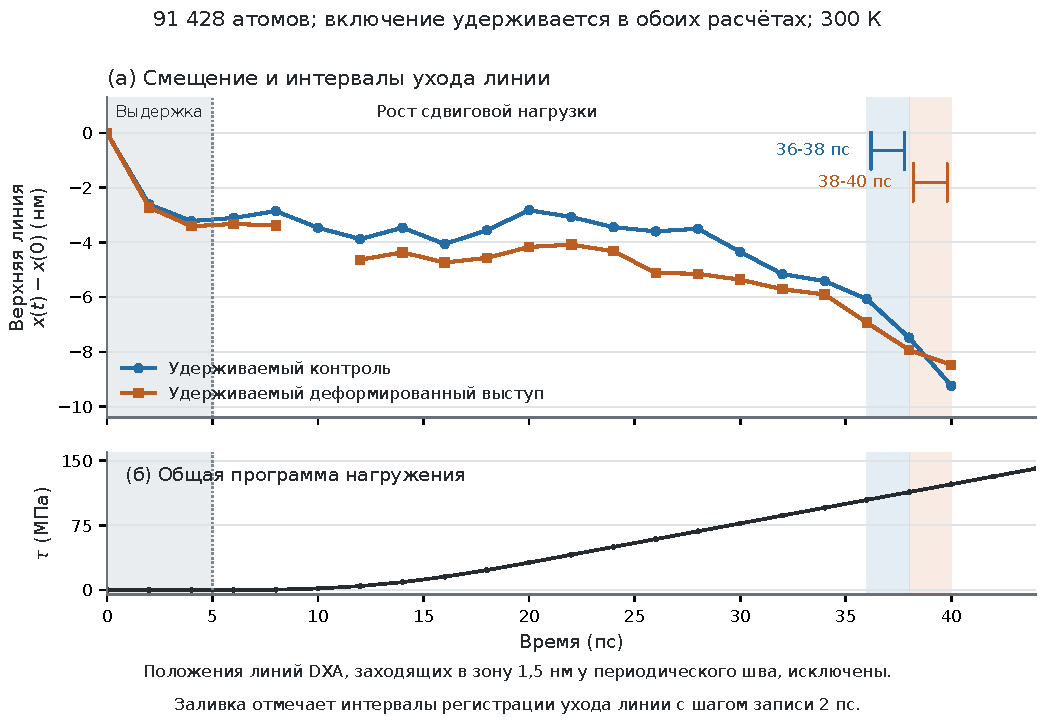
\includegraphics[width=0.96\linewidth]{fig_dynamics_ru.pdf}
\caption{Движение существующих линий в ячейках границы.
Положение верхней линии прослежено при предварительной выдержке
и сдвиговом нагружении вместе с приложенным напряжением.
Контрольная и возмущённая ячейки с удерживаемым включением
пересекают критерий ухода с разницей в один сохранённый кадр.
Начальное движение к выступу и остаточные DXA-сегменты на
периодическом шве ограничивают интерпретацию дальнейших траекторий.
Исчезновение сегмента или изменение его принадлежности
не доказывает образования новой дислокации на границе.}
\label{fig:dynamics}
\end{figure}

Нижняя линия в обеих ячейках с удерживаемым включением
перестаёт выделяться отдельно к 10~пс. Позднее у периодического
шва появляются DXA-сегменты. Их отнесение к исходной линии
только по семейству вектора Бюргерса создало бы ложное позднее
событие ухода. В последнем проанализированном кадре при 44~пс,
около 140{,}9~МПа, в возмущённой ячейке извлечённых сегментов
нет. В контроле остаются три сегмента общей длиной 39{,}3~\AA{}
вблизи $x=7$--10~\AA{}. Поэтому обе конфигурации нельзя
описывать как свободные от дислокаций. Короткие сегменты
учитываются как локальные сигналы DXA без установления механизма
зарождения.

В контроле со свободным включением нижняя линия пересекает
критерий движения между 95{,}5 и 104{,}5~МПа.
Проанализированная траектория продолжается до 395{,}45~МПа
при 100~пс. В этих кадрах не подтверждено возникновение
новой устойчивой дислокации на границе. При более высоких
нагрузках также встречаются короткие сигналы у периодического
шва. Номинальный конец расчёта соответствует 400~МПа
и лежит за последним проанализированным регулярным кадром.
Этот единственный прогон характеризует наблюдавшуюся активность
в заданных граничных условиях, но не определяет универсальный
порог зарождения.

\section{Условная связь с ползучестью}

Последствия полученного масштаба напряжений рассматриваются
в скалярной модели термически активированного скольжения.
Предполагается разреженное распределение компактных частиц
с внешней амплитудой сдвига $\tau(R)=\tau_m(a/R)^3$,
где $R$ отсчитывается от центра частицы.
Положительные и отрицательные локальные напряжения имеют
равные веса, а изменение элементарной термически активированной
скорости описывается множителем
$\cosh(V^*\tau/k_{\mathrm B}T)$ \cite{CaillardMartin2003}.
Активационный объём $V^*$ характеризует чувствительность
барьера к напряжению. Эти предположения дают относительный
прирост скорости
\begin{equation}
H=f x\int_0^x\frac{\cosh u-1}{u^2}\,\mathrm du,
\qquad x=\frac{V^*\tau_m}{k_{\mathrm B}T},
\label{eq:bridge}
\end{equation}
в первом порядке по объёмной доле включений $f$.
Тензорное поле, ориентации зёрен и взаимодействие частиц
при этом сводятся к одной принятой амплитуде.

Для оценки заданы $T=300$~К и $f=0{,}00246$
как представительный разреженный случай.
Целевой прирост $H=0{,}25$ выбран по масштабу
зарегистрированных изменений ползучести.
Чувствительность исследуется в диапазоне
$V^*=19b^3$--$142b^3$. Значение $70b^3$,
полученное для Al--Mg--Si в ином структурном состоянии
\cite{Soula2022JALCOM}, служит ориентиром для этого диапазона.
Из настоящих траекторий активационный объём не определяется.

Выбранная доля примерно соответствует модельному содержанию
0{,}35~мас.\% при принятых плотностях включения и матрицы
3{,}85 и 2{,}70~г/см$^3$. Эти параметры описывают представительное
распределение и имеют собственную неопределённость состава.
Кроме того, $H$ является изменением скорости в активационной
модели. Его связь с накопленной экспериментальной деформацией
требует учесть историю нагружения, для которой применимо такое
описание скорости. Выбор экспериментального изменения в качестве
фиксированного ориентира поэтому добавляет ещё один уровень
моделирования к атомистическому расчёту напряжений.

Решение уравнения~\eqref{eq:bridge} даёт необходимые амплитуды
от 62{,}69 до 8{,}39~МПа по мере роста $V^*$
в выбранном диапазоне (рис.~\ref{fig:bridge}).
При подстановке 15{,}451~МПа в качестве представительной
амплитуды прирост $H=0{,}25$ достигается при
$V^*=77{,}09b^3$. Подстановка 41{,}45~МПа даёт
$28{,}74b^3$. Для этих исходных параметров уточнённый
условный диапазон составляет около 29--77$\,b^3$.
При $V^*=70b^3$ и амплитуде 15{,}451~МПа
получается $H=0{,}156$.

\begin{figure}[!htbp]
\centering
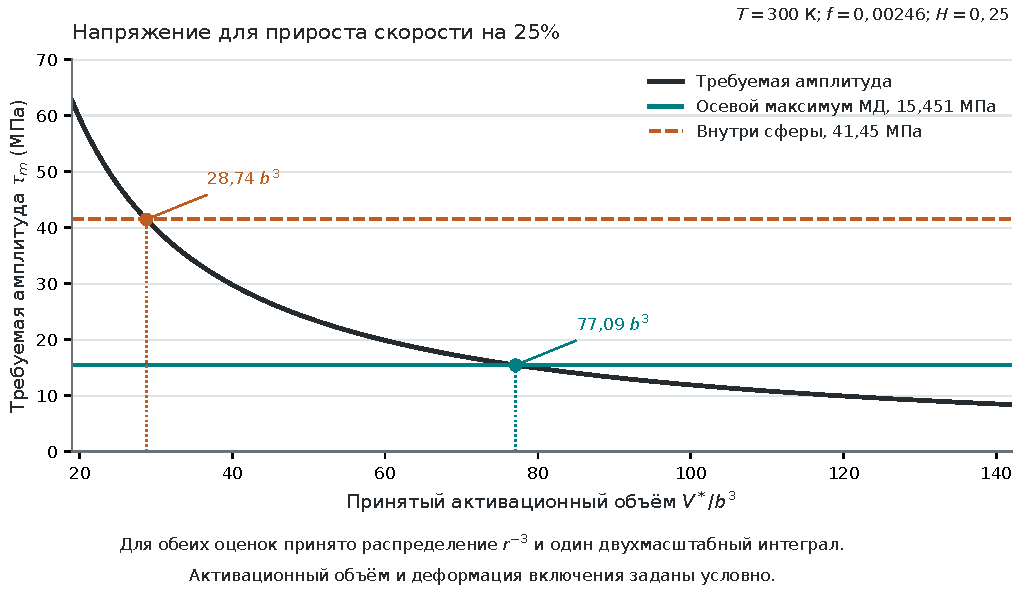
\includegraphics[width=0.92\linewidth]{fig_bridge_ru.pdf}
\caption{Условная оценка термически активированного скольжения
при 300~К и $f=0{,}00246$. Амплитуда сдвига, необходимая
для прироста скорости на 25\%, существенно зависит от
активационного объёма. Значения 15{,}451 и 41{,}45~МПа
служат отдельными иллюстративными входными параметрами
из профиля выступа и внутреннего поля сферы.
Их перенос в скалярную пространственную модель является
дополнительным предположением. Кривая не подогнана
к измеренному активационному объёму или рассчитанной
скорости ползучести.}
\label{fig:bridge}
\end{figure}

Максимум на оси выступа и внутреннее напряжение сферы
относятся к разным физическим и пространственным
определениям. Подстановка каждого из них в
уравнение~\eqref{eq:bridge} показывает последствия
принятой амплитуды, но не устанавливает внешнее
поверхностное напряжение реальных частиц.
Экспоненциальная зависимость от $V^*\tau_m$
позволяет получить целевой прирост при разных
сочетаниях неопределённых входных параметров.
Совпадение при выбранном активационном объёме
поэтому не даёт независимого подтверждения
магнитного механизма.

\section{Обсуждение}

Парный статический расчёт определяет, как конкретная
удерживаемая деформация меняет напряжения матрицы.
Сохранение знака сдвига выявляет противоположные вклады,
скрытые скалярным средним по ширине. Это существенно
при оценке силы на дислокации, положение которой
выделяет лишь часть поля. На высоте, занятой верхней
линией после начальной перестройки, изменение сдвига
в осевом окне составляет около 13--14~МПа.
Его масштаб сопоставим с интервалом между сохранёнными
напряжениями ухода. Для отделения систематического
изменения от чувствительности к начальному состоянию
и идентификации линии нужна серия траекторий.

Интерпретацию ограничивают свойства модели.
Выступ периодически продолжен вдоль направления
линии и опирается на удерживаемый слой.
Он не представляет изолированную частицу
в макроскопическом поликристалле.
Потенциал охватывает необходимые элементы,
однако его переносимость на рассматриваемую границу,
ядра дефектов и взаимодействия с примесями здесь
независимо не проверена. Для экстраполяции
зарегистрированных напряжений ухода отсутствуют
серия размеров ячейки, разные скорости нагружения
и ансамбль начальных скоростей атомов.
Термостат действует во время нагружения, поэтому
расчёты не определяют адиабатический разогрев
или изменения тепловыделения, наблюдаемые в опыте.

Нанометровая протяжённость профиля связана с размерами выступа
и конечной расчётной областью. В упругих решениях для включений
расстояние входит через его отношение к размеру частицы.
Геометрически подобная частица большего размера поэтому может
действовать на большем абсолютном расстоянии при той же
безразмерной деформации. Перенос такого масштабирования
на данный удерживаемый выступ требует дополнительной проверки
геометрии и влияния границ. Один рассчитанный профиль
не устанавливает перекрытия полей включений, разделённых
несколькими микрометрами.

Ячейка сплава даёт дополнительное свидетельство
ограниченной подвижности линии при одном случайном
расположении примесей. За завершённую программу
нагружения до 75~МПа суммарное смещение исследуемой
линии равно 1{,}98~\AA{}, что меньше модуля
вектора Бюргерса. Конфигурация, длительность
наблюдения и внутренние напряжения отличаются
от расчётов границы. Этот результат не определяет
переносимую константу закрепления или калибровку
$V^*$. Траектория, метод анализа и ограничения
сопоставления описаны в дополнительных материалах.

Связь заданной деформации с магнитными свойствами
остаётся самостоятельным вопросом. В исследованиях
Al$_{13}$Fe$_4$ отмечен слабый или необычный
парамагнитный отклик; сильный ферромагнетизм,
предполагаемый для некоторых железосодержащих
включений, ими не установлен
\cite{Albedah2015Mossbauer,Avers2025Crystals}.
Для реальных включений необходимо совместно
определить фазовый состав, магнитный отклик
и изменение формы в поле. Межатомный потенциал
и координатные ограничения не задают магнитного
определяющего соотношения. Поэтому принятая
деформация и рассчитанное напряжение
не являются измерением магнитострикции.

Экспериментальная последовательность задаёт
и временное условие для механизма. Ползучесть
измеряется после магнитной обработки, тогда
как статический расчёт сохраняет механическое
ограничение, а динамические расчёты не воспроизводят
его снятие с последующим отложенным нагружением.
Необратимая перестройка дефектов, остаточная
деформация и изменения распределения препятствий
могут влиять на последующий отклик, но ни один
из этих процессов данным набором записей
не установлен. Результаты определяют механические
величины, которые должно воспроизводить такое
объяснение. Происхождение и время жизни
экспериментальной памяти остаются открытыми.

\section{Заключение}

Удерживаемая деформация 0{,}194\% выступа
Al$_{13}$Fe$_4$ создаёт изменение осевого
касательного напряжения с максимальным модулем
15{,}45~МПа в ячейке границы из 91\,428 атомов.
Пространственная компенсация уменьшает средний
по ширине отклик и меняет его знак.
Модуль осевого сдвига снижается примерно
до 2~МПа на высоте 8{,}6~нм над вершиной.

Парные траектории под нагрузкой показывают
существенное начальное движение существующих
линий и разницу ухода верхней линии в один
сохранённый кадр. Сегменты на периодическом
шве и ограниченный объём наблюдений затрудняют
количественное выделение эффекта.
Отдельный расчёт термически активированного
скольжения выражает чувствительность к принятым
напряжению и активационному объёму.
Вместе эти результаты характеризуют отклик
на удерживаемое механическое ограничение
и определяют пределы его интерпретации как
возможного вклада в магнитно-модифицированную
ползучесть.

\section*{Вклад авторов}

И.\,Е.~Михайловский участвовал в разработке методики
и программного обеспечения, проведении исследования,
формальном анализе, визуализации и подготовке
первоначального текста.
Д.\,Е.~Пшонкин участвовал в разработке концепции,
предоставлении ресурсов, руководстве, рецензировании
и редактировании текста.

\section*{Доступность данных}

В репозитории
\url{https://github.com/iluuua/magnetostriction-plasticity-bounds}
представлены парные статические конфигурации с атомными
вириалами, координатные траектории трёх нагружений ячейки
границы, их начальные и конечные конфигурации и журналы
расчётов. Манифест публикационного набора указывает
сохранённые столбцы траекторий и частоту записи.
Для ячейки сплава доступны полная сохранённая атомистическая
история координат и напряжений, производная таблица положений
из 131 кадра, сводные результаты, начальная и конечная
структуры и журнал расчёта.
Связь представленных величин с архивными записями
описана в дополнительных материалах.

\section*{Доступность кода}

Входные файлы LAMMPS, программа запуска
из опубликованных начальных конфигураций,
код анализа и построения рисунков доступны
в том же репозитории. Манифест публикационного
набора указывает файлы, использованные
для представленных расчётов.

\section*{Конфликт интересов}

Авторы заявляют об отсутствии финансового
конфликта интересов.

\bibliographystyle{unsrtnat}
\bibliography{references}
\end{document}
